\documentclass{article} % Adjust the font scale/size here

\usepackage[portrait, tmargin=0in, bmargin=0in, lmargin=0in, rmargin=0in]{geometry}
\usepackage{graphicx} % Required for including images
\usepackage[normalem]{ulem}
\usepackage{macros}

\usepackage{amsmath} % For typesetting math
\usepackage{amssymb} % Adds new symbols to be used in math mode

\usepackage{booktabs} % Top and bottom rules for tables
\usepackage{enumitem} % Used to reduce itemize/enumerate spacing
\usepackage{palatino} % Use the Palatino font
\usepackage[font=small,labelfont=bf]{caption} % Required for specifying captions to tables and figures

\usepackage{multicol} % Required for multiple columns
\setlength{\columnsep}{1.5em} % Slightly increase the space between columns
\setlength{\columnseprule}{0mm} % No horizontal rule between columns

\usepackage{tikz} % Required for flow chart
\usetikzlibrary{shapes,arrows} % Tikz libraries required for the flow chart in the template

%\usepackage[round]{natbib}   % omit 'round' option if you prefer square brackets
%\bibliographystyle{plainnat}

\begin{document}
\begin{center}
\begin{tikzpicture}
   \begin{axis}[width=\textwidth, height=0.46\textheight,
          %  grid = major,         
            axis y line=middle,
            axis x line=bottom,
						xlabel={$x$},
						every axis x label/.style={at={(current axis.right of origin)},anchor=west},
						ymax=0.5,
						xtick={-1,0,1},
            xticklabels={-1,0,+1},
            yticklabels=\empty
            ]
           \addplot[domain=-2.75:5, green!35!black, thick,smooth] 
              {0.1*(x-1) + 2*0.01*ln(1+exp(-10*(x-1)))} node [pos=0.59,pin={350:\Huge{$f_+$}}] {} ; 
            \addplot[domain=-5:2.75, red!35!black,thick,smooth] 
              {0.1*(x+1) + 2*0.01*ln(1+exp(-10*(x+1)))} node [pos=0.4,pin={215:\Huge{$f_-$}}] {} ; 
   \end{axis}
   \end{tikzpicture}
\end{center}
\vspace{3cm}
\begin{center}
\begin{tikzpicture}
   \begin{axis}[width=\textwidth, height=0.46\textheight,
          %  grid = major,         
            axis y line=middle,
            axis x line=middle,
						xlabel={$x$},
						every axis x label/.style={at={(current axis.right of origin)},anchor=west},
            yticklabels=\empty
            samples = 1000000
            ]
           \addplot[domain=-5:5, green!35!black, thick,smooth] 
              {0.1*(1-exp(-10*(x-1)))/(1+exp(-10*(x-1)))} node [pos=0.59,pin={350:\Huge{$f'_+$}}] {}; 
            \addplot[domain=-5:5, green!35!black, thick,dashed] 
              {
              (x<0)*
              (0.1*(1-exp(-10*(x-1)))/(1+exp(-10*(x-1)))+0.05)
              +
              (x>0)*
              min(0.1*(1-exp(-10*(x+1)))/(1+exp(-10*(x+1)))-0.05,
              0.1*(1-exp(-10*(x-1)))/(1+exp(-10*(x-1)))+0.05)
              } ; 
            \addplot[domain=-5:5, red!35!black,thick,smooth] 
              {0.1*(1-exp(-10*(x+1)))/(1+exp(-10*(x+1)))} node [pos=0.4,pin={135:\Huge{$f'_-$}}] {}; 
              \addplot[domain=-5:5, red!35!black,thick,dashed] 
              {
              (x>0)*
              (0.1*(1-exp(-10*(x+1)))/(1+exp(-10*(x+1)))-0.05)
              +
              (x<0)*
              max(0.1*(1-exp(-10*(x+1)))/(1+exp(-10*(x+1)))-0.05,
              0.1*(1-exp(-10*(x-1)))/(1+exp(-10*(x-1)))+0.05)
              };
   \end{axis}
   \end{tikzpicture}
\end{center}
\end{document}